\section{Methods}
\label{sec:methods}

\subsection{Pipeline Overview}
\label{sec:pipeline}

Our benchmark is built around a modular pipeline that decomposes the materials property prediction task into four independently swappable stages (Figure~\ref{fig:pipeline}).
Given a crystal structure represented as an ASE \texttt{Atoms} object~\cite{larsen2017atomic}, the pipeline proceeds as follows: (i)~a \emph{featurizer} converts the three-dimensional atomic arrangement into a fixed-length numerical vector; (ii)~principal component analysis (PCA) projects this high-dimensional embedding into a reduced subspace; (iii)~a \emph{probabilistic surrogate model} maps the reduced features to a predictive distribution over the target property, yielding both a mean prediction~$\mu(\mathbf{x})$ and an uncertainty estimate~$\sigma(\mathbf{x})$.

The plug-in philosophy is central to our design.
Think of the pipeline like a modular stereo system: the featurizer is the microphone capturing raw signal from crystal structures, PCA is the equaliser compressing it to manageable channels, and the surrogate is the amplifier turning those channels into a useful output.
Any component can be swapped independently, allowing systematic evaluation of all combinations.
We tested 4~microphones $\times$ 3~EQ settings $\times$ 3~amplifiers $\times$ 3~music genres (datasets), totalling 108~unique configurations per dataset.

\begin{figure}[H]
    \centering
    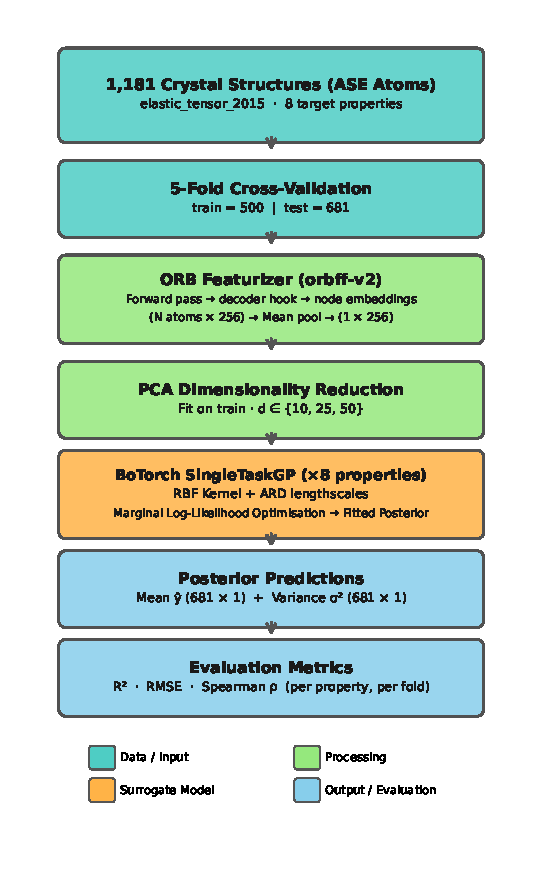
\includegraphics[width=\columnwidth]{figures/fig1_pipeline_schematic.pdf}
    \caption{Modular pipeline for foundation-model-based surrogate modelling. Crystal structures are featurised by one of four embedding methods (SOAP, MACE, ORB, UMA/eSEN), projected to lower dimensions via PCA, and fed into a probabilistic surrogate model (GP, MTGP, or DGP). Each component can be independently swapped, enabling systematic cross-factorial evaluation.}
    \label{fig:pipeline}
\end{figure}


\subsection{Datasets}
\label{sec:datasets}

We evaluate our pipeline on three publicly available datasets from the \texttt{matminer} library~\cite{ward2018matminer}, chosen to span a diverse range of materials properties: mechanical (elastic), electronic (dielectric), and vibrational (phonon).
Table~\ref{tab:datasets} summarises the key characteristics of each dataset.

\begin{table}[H]
    \centering
    \caption{Summary of the three benchmark datasets. All datasets are sourced from \texttt{matminer} and contain DFT-computed properties from the Materials Project~\cite{jain2013materials}.}
    \label{tab:datasets}
    \small
    \begin{tabular}{@{}llcc@{}}
        \toprule
        \textbf{Dataset} & \textbf{Property Type} & \textbf{Structures} & \textbf{Targets} \\
        \midrule
        \texttt{elastic\_tensor\_2015} & Mechanical & $\sim$1{,}181 & 8 \\
        \texttt{dielectric\_constant} & Electronic & $\sim$1{,}056 & 4 \\
        \texttt{phonon\_dielectric\_mp} & Phonon/Electronic & $\sim$1{,}296 & 3 \\
        \bottomrule
    \end{tabular}
\end{table}

\textbf{Elastic tensor dataset}~\cite{deJong2015elastic} contains 1{,}181 inorganic crystalline structures with DFT-computed elastic constants.
We predict 8~target properties: the Voigt, Voigt--Reuss--Hill (VRH), and Reuss averages of both bulk modulus ($K$) and shear modulus ($G$), together with elastic anisotropy and Poisson's ratio.
These properties range from ``easy'' (bulk modulus variants, which depend primarily on bond stiffness and local chemistry) to ``hard'' (elastic anisotropy, which requires capturing directional bonding and crystal symmetry).

\textbf{Dielectric constant dataset}~\cite{petousis2017high} contains approximately 1{,}056 structures with 4~target properties: band gap, refractive index ($n$), and the electronic and total components of the polycrystalline dielectric constant (\texttt{poly\_electronic} and \texttt{poly\_total}).
These properties are sensitive to electronic structure details that are only indirectly captured by geometric embeddings.

\textbf{Phonon dielectric dataset} from the Materials Project contains approximately 1{,}296 structures with 3~target properties: electronic and total dielectric constants (\texttt{eps\_electronic}, \texttt{eps\_total}) and the last phonon density of states peak (\texttt{last\_phdos\_peak}).
The dielectric constants prove extremely challenging for all methods (near-zero \Rtwo{}), while the phonon peak is moderately predictable.


\subsection{Featurizers}
\label{sec:featurizers}

We compare four featurisation strategies spanning the spectrum from classical hand-crafted descriptors to modern foundation model embeddings.
Table~\ref{tab:featurizers} summarises their key architectural differences.

\begin{table*}[!htb]
    \centering
    \caption{Comparison of the four featurisation methods. Foundation model embeddings (MACE, ORB, UMA/eSEN) are extracted from pre-trained models without fine-tuning. The raw embedding dimensionality is reduced via PCA before surrogate training.}
    \label{tab:featurizers}
    \small
    \begin{tabular}{@{}lllcl@{}}
        \toprule
        \textbf{Featurizer} & \textbf{Type} & \textbf{Pre-training Data} & \textbf{Raw Dim.} & \textbf{Key Reference} \\
        \midrule
        SOAP & Classical descriptor & None (analytical) & $\sim$1{,}000+ & Bart{\'o}k \emph{et al.}~\cite{bartok2013representing} \\
        MACE & Foundation model & MPTrj ($\sim$150k structs.) & $\sim$256 & Batatia \emph{et al.}~\cite{batatia2022mace,batatia2024foundation} \\
        ORB & Foundation model & Alexandria + MPTrj ($\sim$120M configs.) & $\sim$256 & Orbital Materials~\cite{orb2024} \\
        UMA/eSEN & Foundation model & Multiple sources & $\sim$256 & Meta FAIR~\cite{uma2025} \\
        \bottomrule
    \end{tabular}
\end{table*}

\textbf{SOAP} (Smooth Overlap of Atomic Positions)~\cite{bartok2013representing} is a classical descriptor that encodes local atomic environments as the power spectrum of a smooth atomic density expanded in radial basis functions and spherical harmonics.
We use the DScribe implementation~\cite{dscribe2020} with standard settings for inorganic crystals.
The structure-level descriptor is obtained by averaging over all atomic environments.
SOAP serves as the classical baseline: it sees only local neighbourhoods within a fixed cutoff radius, analogous to a pinhole camera that captures the immediate scene but misses the wider landscape.

\textbf{MACE}~\cite{batatia2022mace,batatia2024foundation} is an equivariant message-passing neural network that captures many-body interactions through higher-order tensor products.
We extract pooled node embeddings from the pre-trained MACE-MP-0 foundation model~\cite{batatia2024foundation}, which was trained on the MPTrj dataset of $\sim$150{,}000 structures from the Materials Project.
No fine-tuning is performed; the model is used purely as a feature extractor.

\textbf{ORB}~\cite{orb2024} is a graph neural network pre-trained by Orbital Materials on the combined Alexandria and MPTrj datasets, comprising approximately 120~million atomic configurations.
Its graph attention architecture with edge and node features is specifically tuned for periodic crystal structures.
We extract the final-layer embeddings and average over atomic sites.
ORB's large and chemically diverse pre-training corpus gives it broad coverage of the periodic table---analogous to a DSLR camera that captures the full scene with depth of field.

\textbf{UMA/eSEN} (Universal Materials Architecture)~\cite{uma2025} is Meta FAIR's universal interatomic potential based on the eSCN/eSEN architecture.
Pre-trained on multiple data sources spanning diverse chemistries, it represents the most recent generation of universal foundation models.
We extract embeddings analogously to MACE and ORB.


\subsection{Dimensionality Reduction}
\label{sec:pca}

Raw embeddings from all featurisers are projected to lower dimensions via PCA~\cite{jolliffe2002principal} before being passed to the surrogate model.
We evaluate three dimensionality levels: PCA\,=\,10, 25, and 50 components.
PCA serves two purposes: it reduces the computational cost of kernel evaluations in Gaussian processes (which scale cubically with input dimension) and mitigates collinearity among embedding features.
The PCA transformation is fitted on the training set and applied to the test set to prevent data leakage.


\subsection{Surrogate Models}
\label{sec:surrogates}

All surrogate models are implemented in BoTorch~\cite{balandat2020botorch}, built on GPyTorch~\cite{gardner2018gpytorch}, providing a unified framework for comparison.

\textbf{Gaussian Process (GP).}
We use the \texttt{SingleTaskGP} from BoTorch with a Mat{\'e}rn~5/2 kernel and automatic relevance determination (ARD).
Hyperparameters are optimised by maximising the marginal log-likelihood.
The GP is the workhorse of Bayesian optimisation: given a set of observations, it provides a closed-form posterior over the target function with calibrated uncertainty estimates~\cite{rasmussen2006gaussian}.
Each target property is modelled independently.

\textbf{Multi-Task GP (MTGP).}
We use the \texttt{MultiTaskGP} from BoTorch with the intrinsic coregionalisation model (ICM) kernel~\cite{bonilla2007multi}.
The ICM kernel decomposes the multi-output covariance as a Kronecker product of a task correlation matrix and a shared spatial kernel, allowing information to flow between related properties.
Think of it as building one amplifier that shares circuitry between the treble and bass channels, rather than building separate amplifiers for each.
The hypothesis is that correlated properties (e.g., $K_{\text{Voigt}}$, $K_{\text{VRH}}$, $K_{\text{Reuss}}$) should benefit from joint modelling.

\textbf{Deep GP (DGP).}
We use the \texttt{DeepGP} from BoTorch, a two-layer deep Gaussian process~\cite{damianou2013deep} trained via variational inference~\cite{dutordoir2021deep}.
The DGP stacks GP layers to capture non-linear input transformations that a single-layer GP cannot represent.
However, this additional expressiveness comes at the cost of more parameters, potentially more fragile training, and sensitivity to the input dimensionality.


\subsection{Experimental Protocol}
\label{sec:protocol}

We use 5-fold cross-validation with random splits.
For each dataset, we subsample training sets of size $\ntrain \in \{100, 250, 500\}$ from the training fold, while the test fold remains fixed.
This simulates the low-data regime typical of early-stage materials discovery campaigns where DFT calculations are expensive.

The full factorial design yields $4 \times 3 \times 3 \times 3 = 108$ configurations per dataset, times 3~datasets gives 324~configurations.
With 5-fold CV and per-property evaluation (8~properties for elastic, 4 for dielectric, 3 for phonon), the total number of individual model evaluations exceeds 8{,}640.

We report three complementary metrics:
\begin{itemize}[nosep]
    \item \textbf{\Rtwo{}} (coefficient of determination): measures the fraction of variance explained; penalises both bias and scatter.
    \item \textbf{RMSE} (root mean square error): measures absolute prediction error in the units of the target property.
    \item \textbf{Spearman rank correlation} ($\rho$): measures the monotonic relationship between predicted and true values; critical for Bayesian optimisation where we need to correctly \emph{rank} candidates rather than predict exact values.
\end{itemize}
All metrics are computed on the held-out test fold and averaged across folds.
